\section{D-net, Pfeffer observables, and Debnath}
\label{sec:dnet}

The D-net arm imports a reconstructed graph and runs the same two scoring modes on homogeneous conspiracy and mixed identities.
The empirical file is \path{thesisExperiment/data/derived/debnath_hashtag_cascade.json}.
Kind: hashtag co-occurrence.
\texttt{notARetweetCascade: true}.
Nodes are users keyed by published hashtags (63 nodes, 228 directed edges, 171 unique undirected pairs).
Edges reuse a \texttt{retweets[]} container only as a directed-edge slot.
The graph is not a hydrated retweet cascade.
The comparable simulated object is this 63-node custom topology, not the eight 8-node T2 generators.

Hydration of Debnath's tweet identifiers failed.
Mendeley \texttt{10.17632/546hsym93p.1} is an identifier dump, not tweet text \parencite{debnath2023dataset}.
814,924 tweets were not hydrated.
Belief profiles remain theory-faithful reductions, not skip-gram/HDBSCAN centroids \parencite{debnath2023conspiracy,geoeng2023codes}.
Debnath reports no empirical $0$--$5$ \MPR{}.
Simulated auditor \MI{} is therefore not Twitter \MI{} \parencite{ruths2014social}.

Mapping from hashtag cluster to Debnath type was already in the Dnet configs.
No new LLM runs were added for this note.
Empirical cluster identity is conspiracy 28, climate action 19, environmental 14, expert 2.
Mixed Dnet preserves that type mix (conspiracy share $0.444$).
Homogeneous Dnet overwrites every seat to \texttt{conspiracy\_believer} (share $1.0$).
Exact persona-identifier match reconstruct$\leftrightarrow$mixed is 56 of 63; seven seats stay in the same Debnath type on a coarser library id.
Averaged compare \texttt{conspiracyShare=0.722} is H+He pooled and is not a third mix.

\subsection{C5 D-net auditor scores (not pooled into T2)}

\Cref{fig:c5dnet} and \Cref{tab:dnetmpr} list LLM-as-judge headlines on the custom graph.
On D-net, homogeneous conspiracy exceeds mixed identity on both instruments and both seeds.
Continuous SCoPEx: H $1.7349$ versus He $0.9983$.
Continuous chemtrails: H $3.3378$ versus He $2.5068$.
Dual-discrete SCoPEx: H $4.2537$ versus He $2.6880$.
Dual-discrete chemtrails: H $3.7303$ versus He $1.5297$.

That ordering matches composition (D-net H is conspiracy-only).
It does not match the naive eight-topology collapsed He$>$H, which mixed scientists into H.
The H/He label does not travel unchanged onto the 63-node graph.
Dual versus continuous still must not be averaged.
Chemtrails raises continuous \MI{} versus SCoPEx on the same graph; the dual headline does not preserve that article order on He.

\begin{figure}[t]
\centering
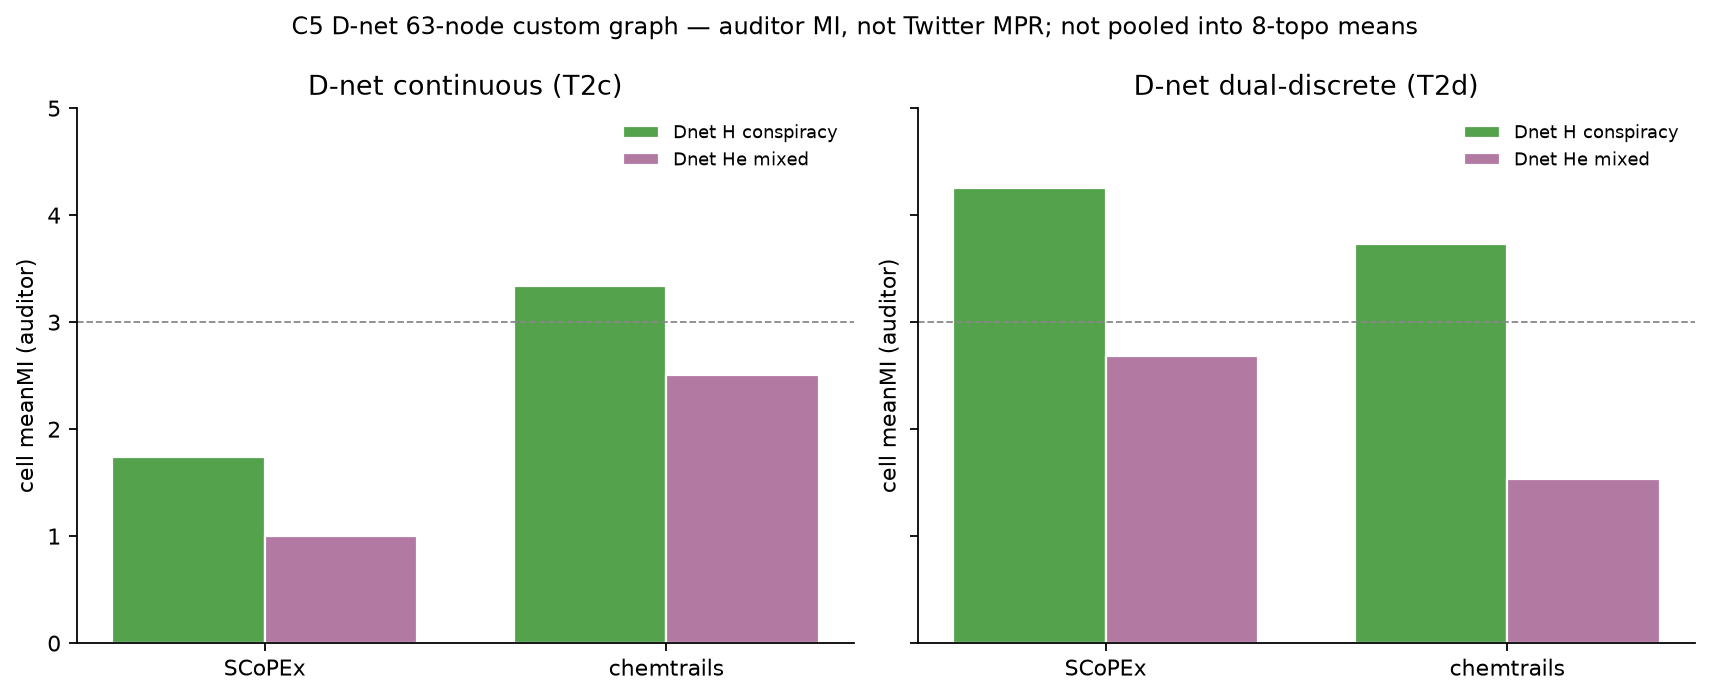
\includegraphics[width=\textwidth]{figures/fig08_c5_dnet.png}
\caption[C5 D-net auditor MI]{C5: D-net 63-node auditor \MI{} by mix, article, and instrument.
Not Twitter \MPR{}.
Not concatenated into the eight T2 topologies.
$N=1$.
Source: \texttt{fig08\_c5\_dnet.png}.}
\label{fig:c5dnet}
\end{figure}

\begin{table}[t]
\centering
\caption{D-net auditor headlines on the hashtag co-occurrence graph.
Sidecar continuous on dual runs is not the T2c headline.}
\label{tab:dnetmpr}
\small
\begin{tabular}{llllr}
\toprule
Run & Article & Mode & Disc.\ \MPR{} & Cont.\ \MPR{} \\
\midrule
Dnet\_c\_H\_conspiracy & SCoPEx & continuous & --- & 1.7349 \\
Dnet\_c\_H\_conspiracy & chemtrails--Gates & continuous & --- & 3.3378 \\
Dnet\_c\_He\_mixed & SCoPEx & continuous & --- & 0.9983 \\
Dnet\_c\_He\_mixed & chemtrails--Gates & continuous & --- & 2.5068 \\
Dnet\_d\_H\_conspiracy & SCoPEx & dual-disc. & 4.2537 & sidecar 2.2495 \\
Dnet\_d\_H\_conspiracy & chemtrails--Gates & dual-disc. & 3.7303 & sidecar 3.1251 \\
Dnet\_d\_He\_mixed & SCoPEx & dual-disc. & 2.6880 & sidecar 1.1302 \\
Dnet\_d\_He\_mixed & chemtrails--Gates & dual-disc. & 1.5297 & sidecar 1.1497 \\
\bottomrule
\end{tabular}
\end{table}

\subsection{Structural comparison}

\Cref{fig:dnet} and \Cref{tab:struct} compare empirical hashtag-graph cascade-shape metrics with the mean of 16 simulated D-net cascades.
Structural similarity (share of compared metrics within a 30\% band) is $0.6885$: breadth matches, depth and structural virality \parencite{goel2016virality} do not.
Kolmogorov--Smirnov tests use $n_{\mathrm{real}}=1$ and $n_{\mathrm{sim}}=16$ and are underpowered.
DTFS $=0.2754$ with \texttt{isValidated=false} (threshold $0.70$).
That table is cascade shape, not a Pfeffer factor.

Empirical transitivity is $0.315$; mean local clustering is $0.515$; the chemtrails hub has 33 unique neighbours.
D-net copies that graph; it does not grow clusters.
On 171 unweighted unique-undirected pairs, the binary conspiracy cut has Newman--Girvan $Q=0.4297$ under mixed labels.
The homogeneous assignment is one community and therefore has $Q=0$.
The six assigned graph clusters instead have $Q=0.5489$; modularity of a label partition is not a clustering coefficient.

\begin{figure}[t]
\centering
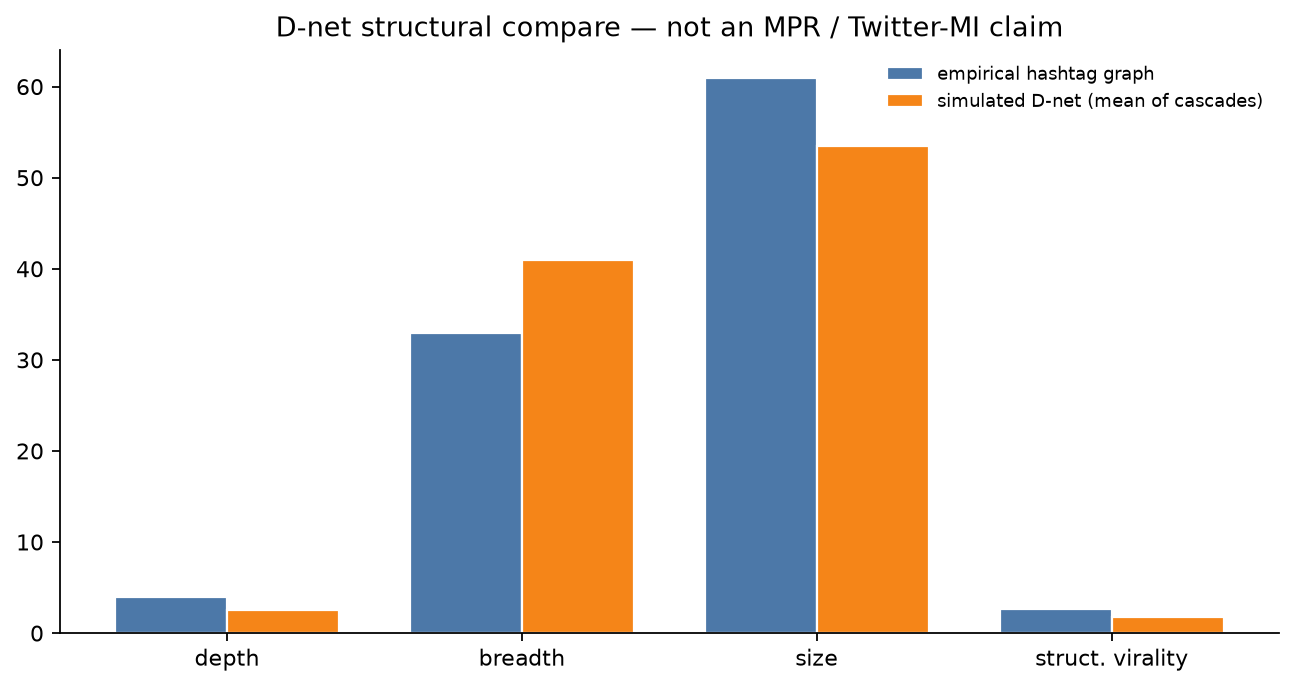
\includegraphics[width=0.88\textwidth]{figures/fig09_dnet_structural.png}
\caption[D-net structural compare]{Empirical hashtag-graph metrics versus mean simulated D-net metrics (16 cascades).
This is a structural comparison, not an \MPR{} or Twitter-\MI{} claim.
Source: \texttt{fig09\_dnet\_structural.png}.}
\label{fig:dnet}
\end{figure}

\begin{table}[t]
\centering
\caption{D-net structural metrics.
Match $=$ within a 30\% band of the empirical value.
KS/JS: $n_{\mathrm{real}}=1$, underpowered.}
\label{tab:struct}
\small
\begin{tabular}{lrrll}
\toprule
Metric & Emp. & Sim.\ mean & Match (30\%) & Note \\
\midrule
depth & 4 & 2.5625 & no & longest path from root \\
breadth & 33 & 40.9375 & yes & max nodes at one level \\
size & 61 & 53.5 & --- & informational \\
struct.\ virality & 2.7 & 1.7963 & no & \textcite{goel2016virality} \\
speed & n/a emp. & 8 ticks & --- & do not convert ticks to hours \\
mean \MI{} & no emp.\ \MPR{} & 2.5529 & do not equate & auditor only \\
\bottomrule
\end{tabular}
\end{table}

\subsection{Pfeffer 2014: seven factors, then a remapping}

\textcite{pfeffer2014firestorms} list seven interrelated factors in the Outlook section:
\begin{enumerate}[nosep]
\item speed and volume of communication;
\item binary choices (like/share/retweet as either--or);
\item network clusters;
\item unrestrained information flow;
\item lack of diversity;
\item cross-media dynamics;
\item network-triggered decision processes.
\end{enumerate}
That list is the primary theory.
The thesis six-knob vocabulary is a computational remapping, not a restatement of the 2014 paper.
\Cref{tab:pfeffer} splits homogeneous from mixed simulation so that homophily $1.0$ is not pooled as a third mix.

Identity-edge homophily on the empirical graph is $0.873$ (BP-family $0.838$).
Mixed Dnet reproduces block echo (identity homophily $0.838$).
Homogeneous Dnet reports homophily $1.0$ because identity was erased.
The earlier harvest row that averaged H+He into \texttt{edgeHomophily=1} is a homogeneous artefact.

Binary choices (Outlook \#2) have no engine row.
Scored actions are ternary, with reinterpret about $0.46$--$0.53$.
That pattern is the opposite of limited like/share interaction.
Cross-media (Outlook \#6) remains held: no broadcast agent.
Surprise is held drip from \texttt{user\_chemtrails\_hub}.
Temporal series are not available empirically; the sim clock is eight ticks, and 61 of 63 nodes are reached in all four primary cells.
Outlook \#4 (hundreds to thousands of weak ties) is not this 63-node hub of degree 33.

\begin{table}[t]
\centering
\caption{Pfeffer observables on the Debnath hashtag fallback versus simulated D-net, H and He split.
Empirical valence is a toxicity/hashtag proxy, not \MPR{}.
Simulated \MI{} is an auditor score, not Twitter \MI{}.}
\label{tab:pfeffer}
\scriptsize
\begin{tabular}{>{\raggedright\arraybackslash}p{0.14\textwidth}
                >{\raggedright\arraybackslash}p{0.20\textwidth}
                >{\raggedright\arraybackslash}p{0.28\textwidth}
                >{\raggedright\arraybackslash}p{0.26\textwidth}}
\toprule
Observable & Pfeffer 2014 map & Empirical & Simulated (split) \\
\midrule
valence & affective character (definition), not an Outlook number & hashtag prior $0.1097$; paper toxicity mean $0.17$ & auditor \MI{}; chemtrails $>$ SCoPEx on continuous H and He \\
surprise & \#1 speed/volume (shock vs drip) & paper SCoPEx spike; not reconstructed & held drip from chemtrails hub \\
identity & \#5 lack of diversity & conspiracy share $0.444$ & H $1.0$; He $0.444$; do not pool to $0.722$ \\
clustering & \#3 network clusters & transitivity $0.315$; local $0.515$; graph-cluster $Q=0.5489$ & same topology; conspiracy-cut $Q=0.4297$ mixed, one-community $Q=0$ \\
echo & \#3 + \#4 + parts of \#5 & identity homophily $0.873$ & He $0.838$; H $1.0$ by construction \\
temporal & \#1 / \#7 & not available (no tweet clock) & 8 ticks; 61/63 nodes reached \\
cross-media & \#6 & held & held (no engine knob) \\
binary choices & \#2 (no thesis knob) & no like/retweet actions & ternary rewrite, not Schelling binary \\
\bottomrule
\end{tabular}
\end{table}

The table is an honesty ledger, not a seven-factor confirmation.
Clustering here is an empirical-structure result copied into D-net.
Echo is label-dependent.
Surprise, temporal acceleration, and cross-media were held or missing empirically.
